\chapter{Resultados}\label{Resultados}

Neste capítulo serão apresentados os resultados obtidos segundo a formulação dos Capítulos \ref{Transferência} e \ref{Metodologia}. Tais resultados serão discutidos e comentados, e também comparados com a literatura para obter-se validez.

\section{Troca de Coordenadas na posição 1 (Alinhado)}
No que diz respeito a posição do celular alinhado com as coordenadas do carro, foi observado a correlação alta (Figura \ref{fig:hmapTrip1}) entre os eixos. O que era esperado uma vez que a matriz de rotação nesse caso especifico se trata da matriz identidade. Ou seja, ao aplicada a matriz de rotação não deve haver alteração nas medições observadas.


\begin{figure}
    \centering
    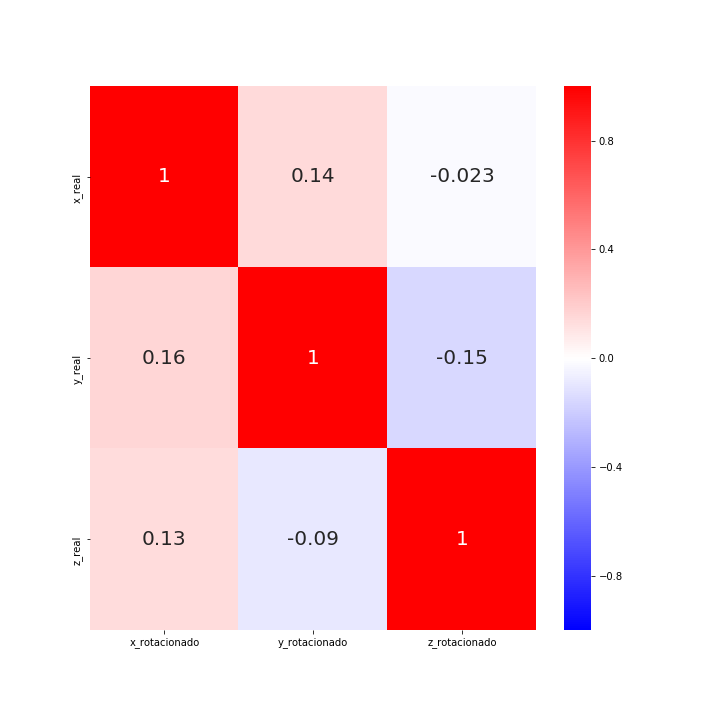
\includegraphics[width=100mm]{Figuras/hmaptrip1.png}
    \caption{Correlação entre os eixos, posição 1.}
    \label{fig:hmapTrip1}
\end{figure}{}
 
\begin{figure}
    \centering
    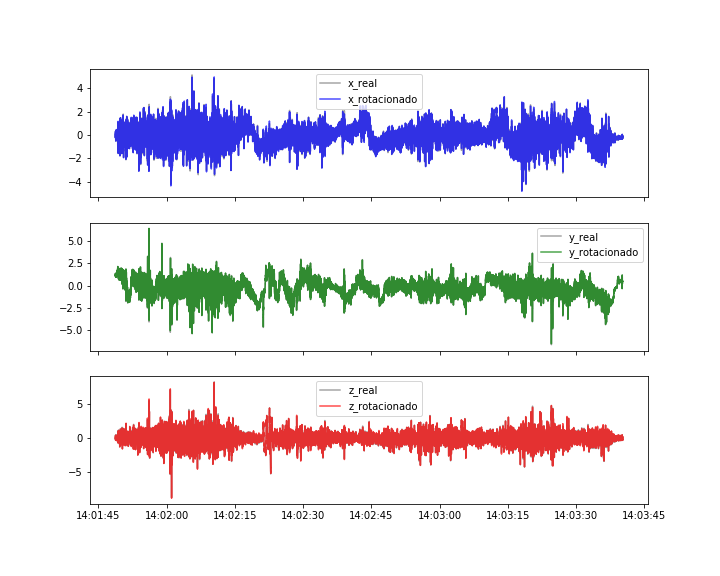
\includegraphics[width=150mm]{Figuras/realrotacionadotrip1.png}
    \caption{Correlação entre os eixos, posição 1.}
    \label{fig:realrotacionadoTrip1}
\end{figure}{}
 
\section{Troca de Coordenadas na posição 2 (Deitado)}
Para o caso do celular deitado, foi identificada uma correlação positiva entre o eixo X do aparelho e Y do carro; seguida de uma correlação negativa entre o X do carro e o Y do celular e positiva entre o eixo Z de ambos, conforme pode ser observado nas Figuras \ref{fig:hmapTrip2} e \ref{fig:realrotacionadoTrip2}.

\begin{figure}
    \centering
    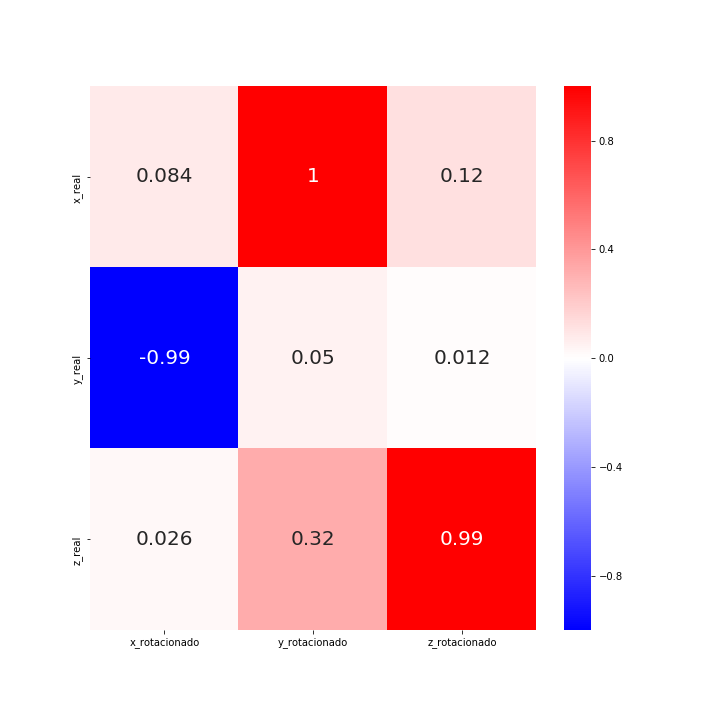
\includegraphics[width=100mm]{Figuras/hmaptrip2.png}
    \caption{Correlação entre os eixos, posição 1.}
    \label{fig:hmapTrip2}
\end{figure}{}
 
\begin{figure}
    \centering
    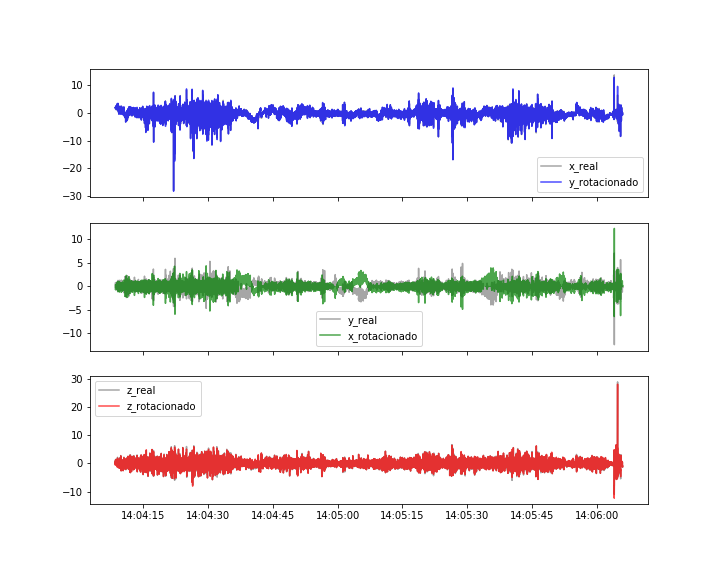
\includegraphics[width=150mm]{Figuras/realrotacionadotrip2.png}
    \caption{Correlação entre os eixos, posição 1.}
    \label{fig:realrotacionadoTrip2}
\end{figure}{}

\section{Troca de Coordenadas na posição 3 (Caso Genérico)}
Em termos do caso genérico, não é trivial observar se a rotação foi bem sucedida apenas observando-se a correlação entre os eixos. Nesse sentido, utilizou-se uma abordagem indireta. Onde, primeiramente se observou o quanto de energia (nesse caso em termos da variância) estava concentrada em cada eixo. Uma vez que o percurso foi o mesmo, e foi realizada em condições parecidas, os resultados do dado rotacionado devem convergir. Tal comportamento pode ser comprovado de acordo com a Tabela \ref{tab:qtdEnergiaPorEixo}. 


\begin{table}[]
\caption{Quantidade de Energia por Eixo Rotacionado}
\label{tab:qtdEnergiaPorEixo}
\begin{tabular}{cccc}
\hline
\textbf{Posição} & \textbf{\% Energia em X} & \textbf{\% Energia em Y} & \textbf{\% Energia em Z} \\ \hline
1 (Alinhado) & 31.42 & 63.98 & 4.60 \\
2 (Deitado) & 34.67 & 60.46 & 4.86 \\
3 (Genérico) & 28.78 & 63.61 & 7.61 \\ \hline
\multicolumn{4}{c}{Fonte: Próprio Autor a partir dos dados coletados}
\end{tabular}
\end{table}

No entanto, somente o quantidade de energia não basta, porque ela apresentaria a mesma proporção caso o sentido dos vetores estimado na matriz de rotação fosse contrário. Com isso em vista, lançou-se mão de o percurso em que se realizou o experimento ser conhecido. Nesse caso, existem 4 curvas a direita no percurso, e estas devem possuir assinaturas distintas tanto no eixo X do acelerômetro rotacionado quanto no eixo Z do giroscópio. 

Devido ao fato do giroscópio medir a velocidade angular no eixo. Ele vai apresentar sinal negativo em Z quando uma curva for para direita (sentido horário do carro) e positiva para esquerda (sentido horário). Por outro lado, no eixo X do acelerômetro (que se refere a aceleração lateral) o valor é positivo no caso de uma curva a direita e negativo para uma curva a esquerda.

Tal comportamento pode ser observado nas três corridas conforme explicitado pela Figura \ref{fig:assinaturaCurvas}. Assim confirmando que a troca de base foi realizada através do método proposto, de forma bem sucedida em todos os três casos.

\begin{figure}
    \centering
    \subfloat[Posição 1 (Alinhado).]{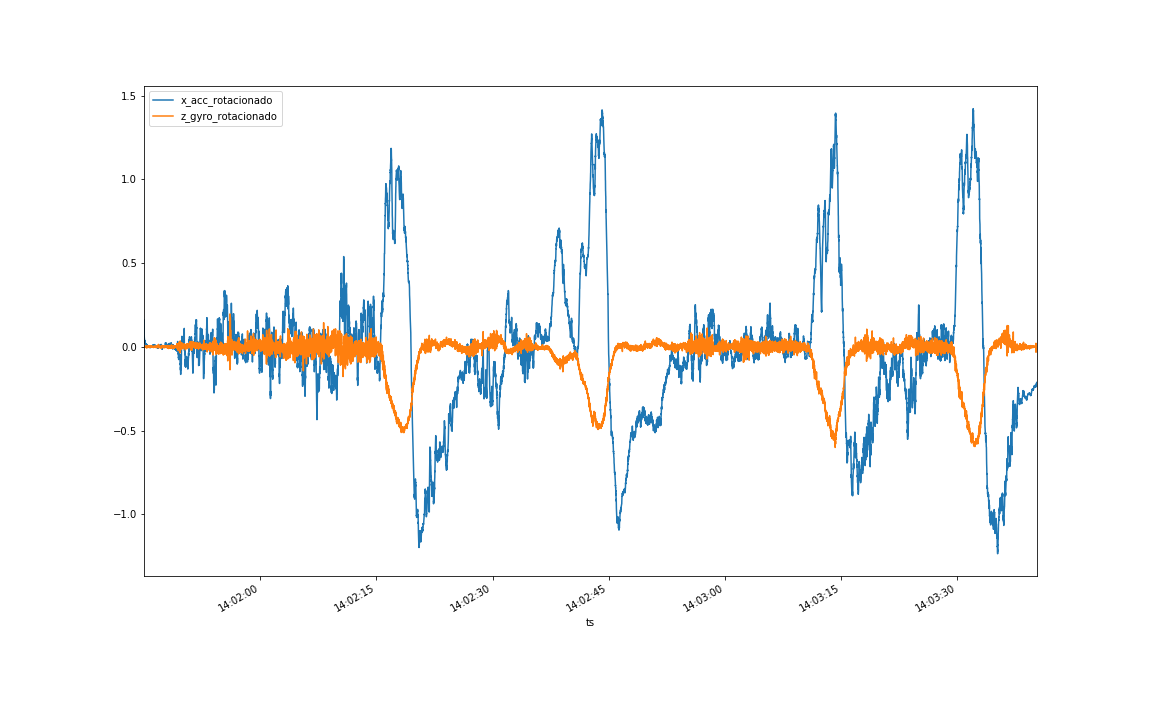
\includegraphics[height=50mm,width=\textwidth]{Figuras/curvaDireitatrip1.png}}
    \\
    \subfloat[Posição 2 (Deitado).]{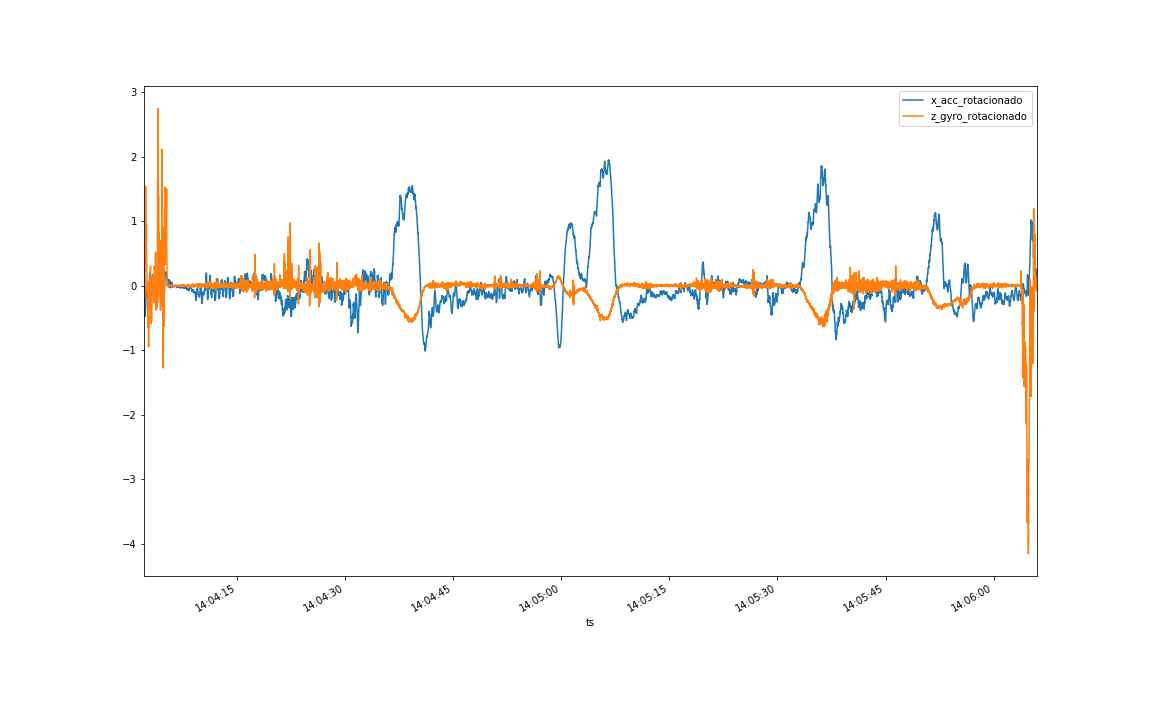
\includegraphics[height=50mm,width=\textwidth]{Figuras/curvaDireitatrip2.png}}
    \\
    \subfloat[Posição 3 (Genérica).]{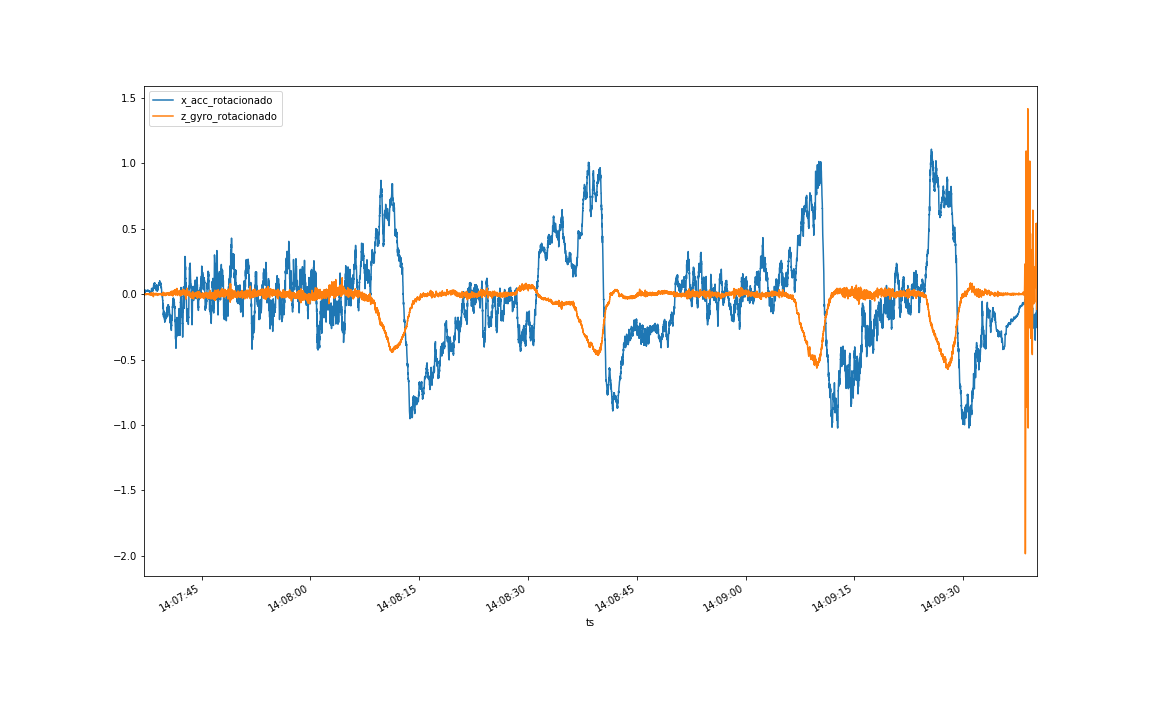
\includegraphics[height=50mm,width=\textwidth]{Figuras/curvaDireitatrip3.png}}
    \caption{Assinatura de curva nas diferentes posições}
    \label{fig:assinaturaCurvas}
\end{figure}{}

\citeauthor{zheng2016unsupervised} afirma que em estudos naturalísticos de direção, as manobras são geralmente anotadas manualmente e avaliadas de forma subjetiva através da revisão de vídeos. 

Uma vez que se possui o dado rotacionado, esse tempo pode ser reduzido através da detecção de eventos simples de direção.

Com o dado rotacionado, pode-se enfim, conforme visto em trabalho anteriores (\citep{zheng2016unsupervised}, \citep{Paefgen:2012:DBA:2406367.2406412} , \cite{fazeen2012safe}) através de limiares heurísticos, detectar eventos simples a respeito das corridas, de forma não supervisionada, facilitando assim o trabalho de classificação. 

De forma a realizar esse classificação não supervisionada, se utilizou os limiares presentes em \citep{Paefgen:2012:DBA:2406367.2406412} em conjunto com a conclusão de \cite{zheng2015mobileutdrive} a respeito da correlação alta entre o giroscópio e o manobrar do volante. De tal maneira que se pode classificar corretamente curvas, acelerações e desacelerações em todos os três casos (Figuras \ref{fig:eventosTrip1},\ref{fig:eventosTrip2},\ref{fig:eventosTrip3}).

\begin{figure}
    \centering
    \subfloat[Eventos no eixo $y$ do acelerômetro rotacionado.]{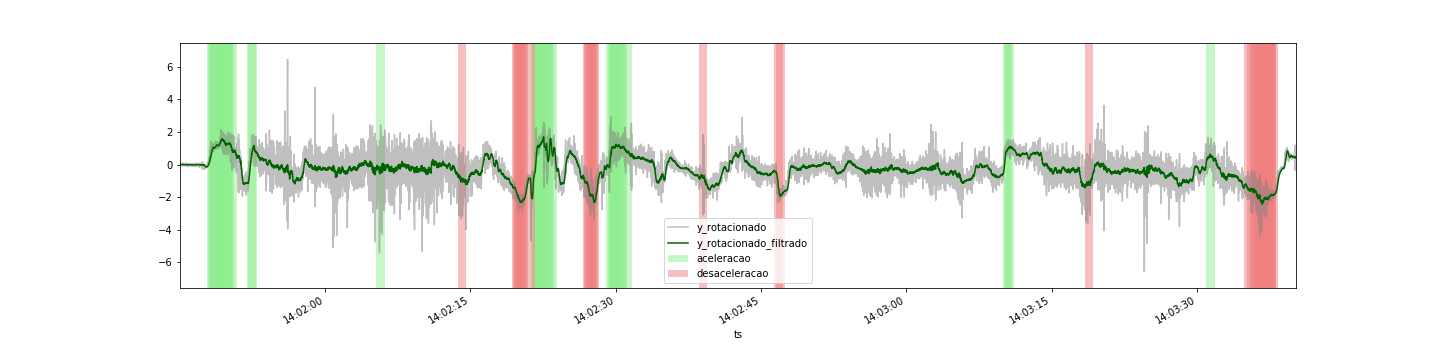
\includegraphics[height=70mm,width=\textwidth]{Figuras/eventosYtrip1.png}}
    \\
    \subfloat[Eventos no eixo $x$ do acelerômetro rotacionado e $z$ do giroscópio rotacionado.]{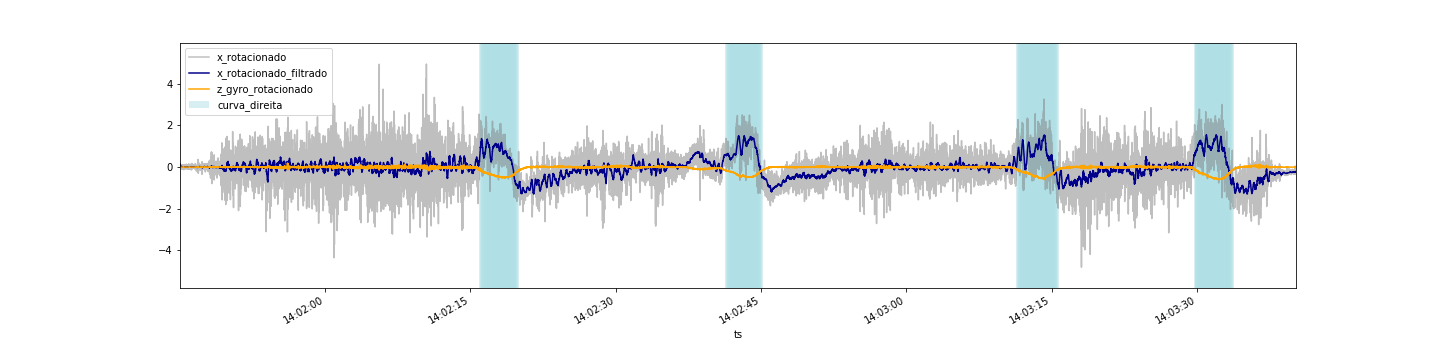
\includegraphics[height=70mm,width=\textwidth]{Figuras/eventosXGtrip1.png}}
    \caption{Assinatura de Eventos - Posição 1}
    \label{fig:eventosTrip1}
\end{figure}{}

\begin{figure}
    \centering
    \subfloat[Eventos no eixo $y$ do acelerômetro rotacionado.]{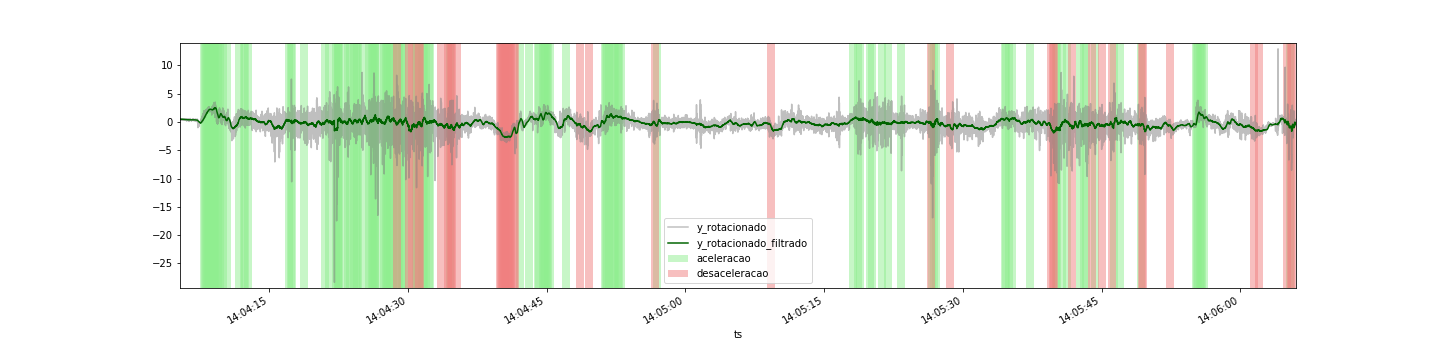
\includegraphics[height=70mm,width=\textwidth]{Figuras/eventosYtrip2.png}}
    \\
    \subfloat[Eventos no eixo $x$ do acelerômetro rotacionado e $z$ do giroscópio rotacionado.]{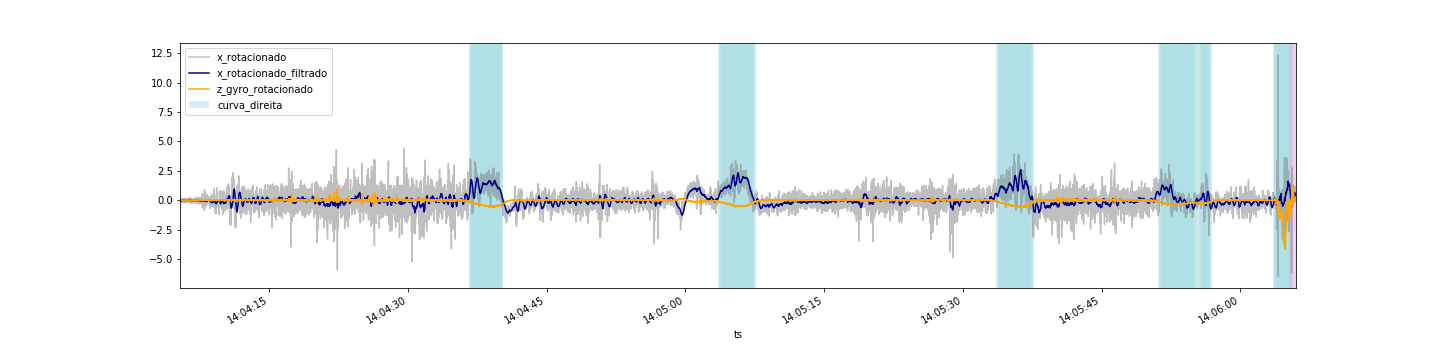
\includegraphics[height=70mm,width=\textwidth]{Figuras/eventosXGtrip2.png}}
    \caption{Assinatura de Eventos - Posição 2}
    \label{fig:eventosTrip2}
\end{figure}{}


\begin{figure}
    \centering
    \subfloat[Eventos no eixo $y$ do acelerômetro rotacionado.]{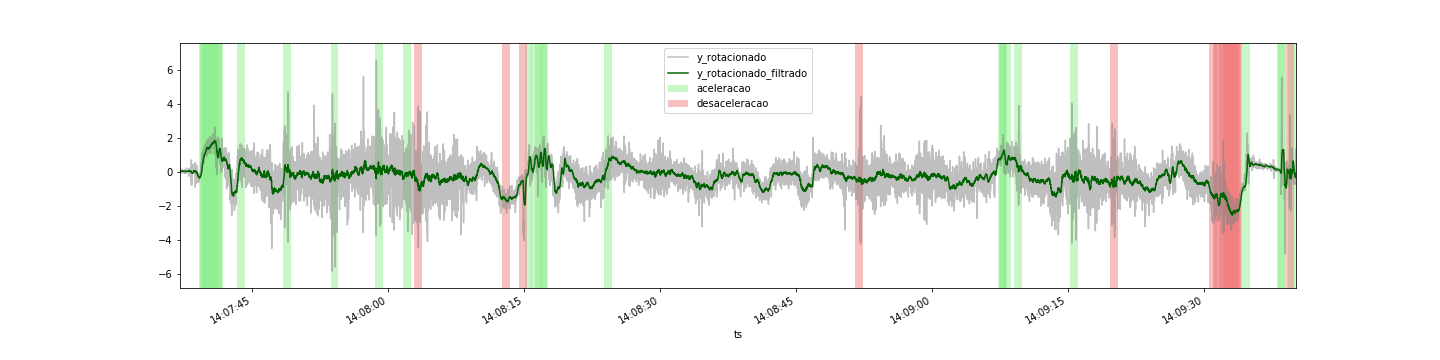
\includegraphics[height=70mm,width=\textwidth]{Figuras/eventosYtrip3.png}}
    \\
    \subfloat[Eventos no eixo $x$ do acelerômetro rotacionado e $z$ do giroscópio rotacionado.]{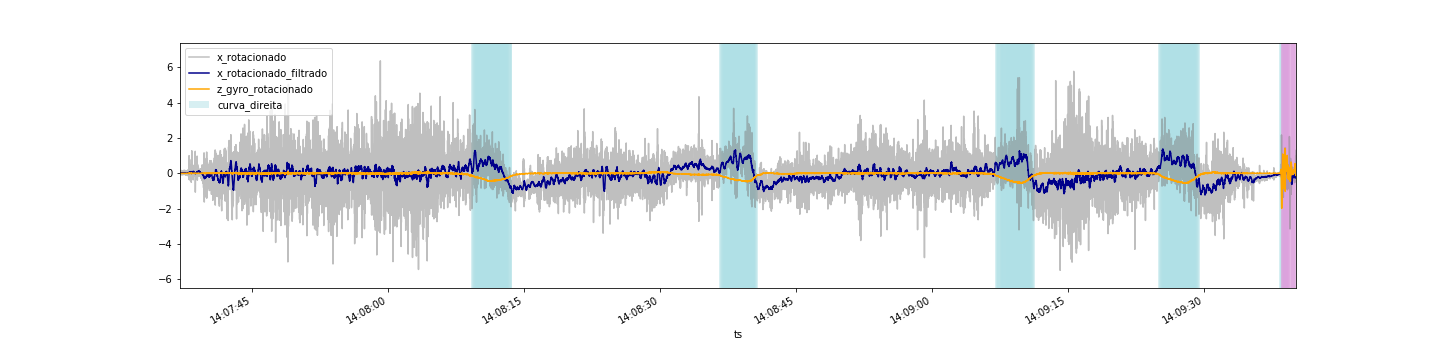
\includegraphics[height=70mm,width=\textwidth]{Figuras/eventosXGtrip3.png}}
    \caption{Assinatura de Eventos - Posição 3}
    \label{fig:eventosTrip3}
\end{figure}{}


